\documentclass[11pt]{article}
\usepackage{fullpage}
\usepackage{graphicx}
\usepackage{float}
\usepackage{tikz}
\usetikzlibrary{matrix,calc}
\usepackage{amsmath}
%opening
\title{\textbf{Homework 1}}
\author{Adam Sumner \\ ECE 429}
\date{September 21st, 2015}

\begin{document}

\maketitle

\section{Explain the Following Terminologies Briefly}

\begin{itemize}
	\item \textbf{Moore's Law} - The observation that the number of transistors in dense integrated circuits has doubled approximately every two years. Named after Gordan E. Moore
	\item \textbf{Feature Size} - The minimum dimension of a transistor that can be reliably built
	\item \textbf{VLSI Design for Power} - Discipline of design that aims to reduce power dissipations while maintaining adequate throughput rate
	\item \textbf{VLSI Design for Manufacturing} - Discipline of design that aims to produce a product in a timely manner with sufficient yield to be profitable
	\item \textbf{ASIC} - Application-Specific Integrated Circuit. An integrated circuit customized for a particular use, rather than general-purpose use
	\item \textbf{Logical Synthesis} - Process by which an abstract from of circuit behavior (usually represented at RTL) is turned into a design implementation
	\item \textbf{Physical Synthesis} - Step in the design cycle that converts circuit representations of components into geometric representations of shapes which, when they are manufactured in their corresponding layers, will ensure the correct functionality
	\item \textbf{Dynamic Power and Leakage Power} - The power consumed during the switching of a transistor, and the power lost to leakage current of transistors
	\item \textbf{Conduction Band} - The lowest range of vacant electronic states. Determines conductivity of the solid
	\item \textbf{Valence Band} - The highest range of electron energies in which electrons are normally present at absolute zero. Determines conductivity of the solid
	\item \textbf{Velocity Saturation} - Sate of a semiconductor when the carrier velocity reaches a maximum value
	\item \textbf{Subthreshold Conduction} - The current between the source and drain of a MOSFET when the transistor is in the subthreshold region
	\item \textbf{Hot Carriers} - Electrons in a solid-state electronic device that gains sufficient kinetic energy to overcome a potential barrier in order to break an interface state
	\item \textbf{MOSFET Operation Regions} - Three separate modes of a MOSFET depending on the voltage at the terminals: Cutoff, Triode, and Saturation
\end{itemize}

\section{Exercise 1.5}
\begin{figure}[H]
\centering
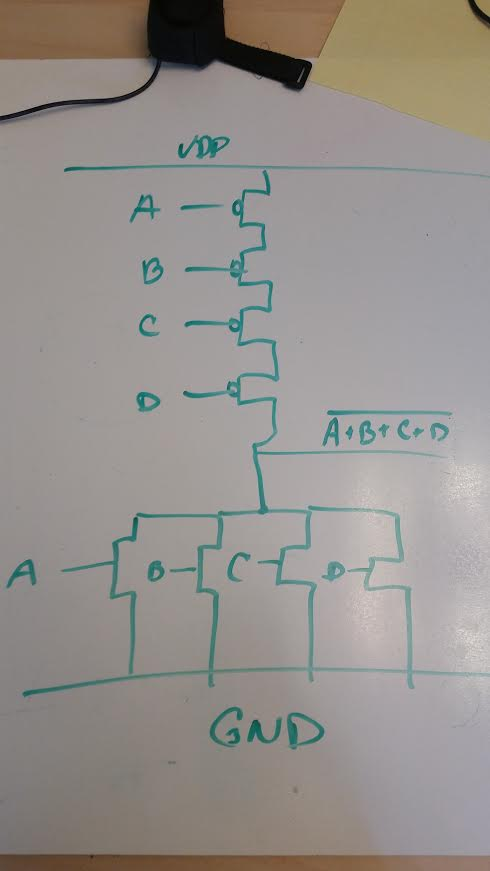
\includegraphics[width=0.5\linewidth]{1-5.jpg}
\caption{4 Input NOR Gate}
\label{fig:1.5}
\end{figure}

\section{Exercise 1.3}
a)
\begin{figure}[H]
\centering
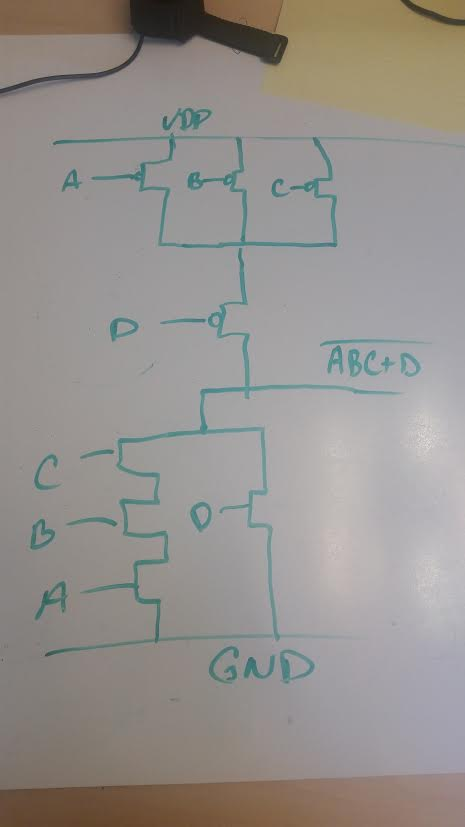
\includegraphics[width=0.5\linewidth]{1-6a}
\caption{$\overline{ABC+D}$}
\label{fig:1.6a}
\end{figure}
b)
\begin{figure}[H]
\centering
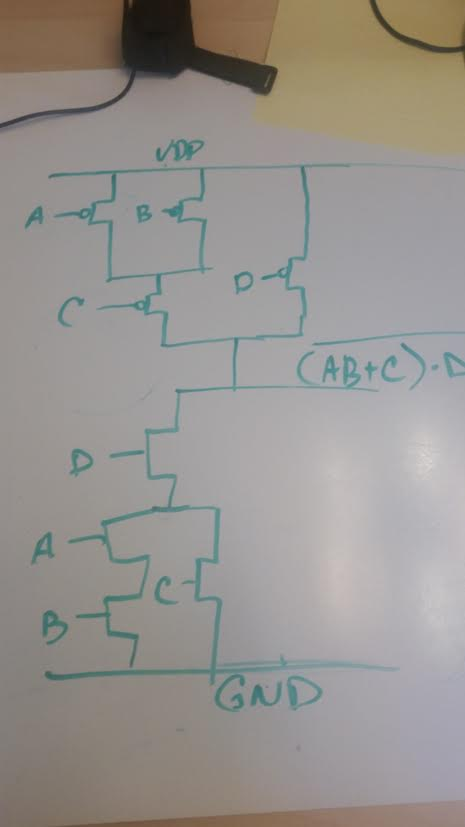
\includegraphics[width=0.5\linewidth]{1-6b}
\caption{$\overline{(AB+C)\cdot D}$}
\label{fig:1-6b}
\end{figure}
c)
\begin{figure}[H]
\centering
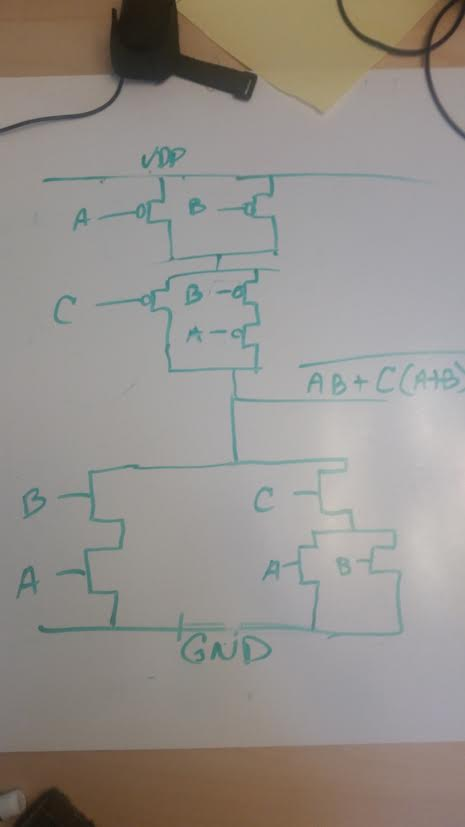
\includegraphics[width=0.5\linewidth]{1-6c}
\caption{$\overline{AB+C(A+B)}$}
\label{fig:1-6c}
\end{figure}
\section{Exercise 1.10}
\begin{figure}[H]
\centering
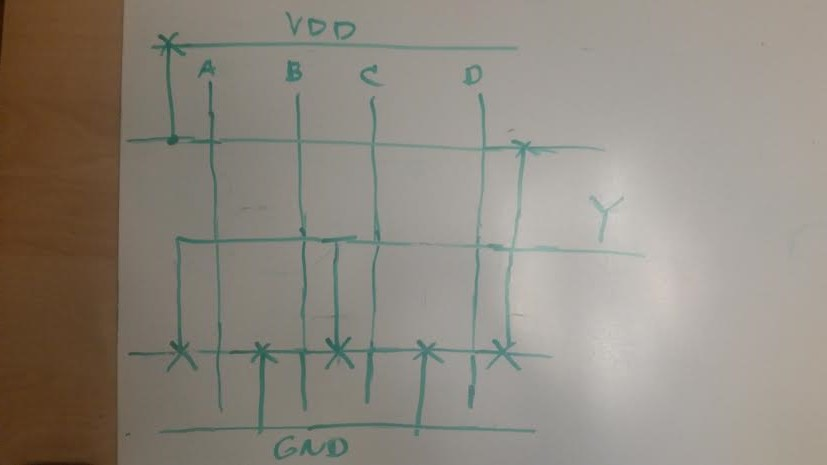
\includegraphics[width=1\linewidth]{1-10}
\caption{Stick Diagram for 4 Input NOR Gate}
\label{fig:1-10}
\end{figure}
\section{Exercise 2.2}
Shockley Equation: 
\begin{equation*}
I_{ds} = \begin{cases}


	 0   &V_{gs} < V_t \quad \quad \textrm{Cutoff}\\
	 \mu C_{ox} \frac{W}{L}(V_{GT} - 0.5V_{ds})V_{ds} & V_{ds} < V_{dsat} \quad \textrm{Linear} \\
	 \mu C_{ox} \frac{W}{2L}V_{GT}^2 & V_{ds} > V_{dsat} \quad \textrm{Saturation}
\end{cases}
\end{equation*}
Assuming the linear region, the current through the bottom transistor is:
\begin{align*}
	I_{ds2} & = \mu C_{ox} \frac{W}{L}(V_{GT} - 0.5V_{ds})V_{ds}\\
	& = \mu C_{ox} \frac{W}{L}(V_{DD} - V_t - 0.5V_{1})V_{1}
\end{align*}
The current through the top transistor is:
\begin{align*}
	I_{ds2} & = \mu C_{ox} \frac{W}{L}(V_{GT} - 0.5V_{ds})V_{ds}\\
	& = \mu C_{ox} \frac{W}{L}(V_{DD} - V_1 -V_t - 0.5(V_{ds} -V_{1}))(V_{ds} -V_{1})
\end{align*}
\\
Solving for $V_1$, where $V_1$ is the voltage between the top and bottom transistors, we can obtain a quadratic expression:

\begin{align*}
		\mu C_{ox} \frac{W}{L}(V_{DD} - V_t - 0.5V_{1})V_{1} &= \mu C_{ox} \frac{W}{L}(V_{DD} - V_1 - V_t - 0.5(V_{ds} -V_{1}))(V_{ds} -V_{1})\\
		(V_{DD} - V_t - 0.5V_{1})V_{1} &= (V_{DD} - V_1 -V_t - 0.5(V_{ds} -V_{1}))(V_{ds} -V_{1})\\
		(V_{DD}-V_t)V_1-0.5V_1^2 &= (V_{DD}-V_t -0.5V_{ds})+0.5V_1^2-V_1(V_{DD}- V_T)\\
		0 &= V_1^2 - 2V_1(V_{DD} - V_t)+ V_{ds}(V_{DD}-0.5V_{ds} -V_t)\\
		V_1&= \frac{2(V_{DD}-V_t)\pm \sqrt{4(V_{DD}-V_t)^2-4V_{ds}(V_{DD}-0.5V_{ds}-V_t)}}{2}	
\end{align*}
	Plugging $V_1$ into the original equation and doing a lot of tedious calculations we get:
	$$I_{ds2} =  \mu C_{ox} \frac{W}{2L}(V_{DD}-V_t-0.5V_{ds})V_{ds}$$
~\\	
	The equation for $I_{ds1}$ is:
	$$I_{ds1} =  \mu C_{ox} \frac{W}{2L}(V_{DD}-V_t-0.5V_{ds})V_{ds}$$
~\\	
Therefore the two currents are equivalent
\section{Exercise 2.3}
$I_{ds2}$ will be less than $I_{ds1}$ because in the case of having one transistor, $V_{sb} = 0$, however, when two transistors are in use, there is a voltage $V_{sb} \ne 0$ in the top transistor. The body effect will cause the threshold voltage to be greater than $V_{to}$, thus resulting in a lower value of $I_{ds2}$.
\section{Exercise 2.7}
Body Effect: $$V_t = V_{to}+ \gamma (\sqrt{\phi _s + V_{sb}} - \sqrt{\phi _s})$$
$$\gamma = \frac{t_{ox}}{\epsilon _ {0} k_{ox}} \sqrt{2q \epsilon _{si} N_A}$$
$$\phi _s = 2 v_T \textrm{ln}(\frac{N_A}{n_i})$$
Solving for $\gamma$ and $\phi _s$:
$$\phi _s = 2(0.026)\textrm{ln}\frac{2 \times 10^{17} ~\textrm{cm}^{-3}}{1.45 \times 10^{10}~\textrm{cm}^{-3}} \approx 0.8548$$
$$\gamma = \frac{100 \times 10^-8}{3.9 \cdot 8.85 \times 10^{-14}}\sqrt{2(1.6 \times 10^{-19})(11.7)(8.85 \times 10^{-14})(2 \times 10^{17})} \approx 0.7458$$
Solving for the new threshold voltage we get:
$$V_t = 0.7 + 0.7458(\sqrt{0.8548 +4} -\sqrt{0.8548}) \approx 1.653\textrm{V}$$
The voltage level changes by 0.95V
\section{Exercise 2.9}
A negative substrate bias should be used
\section{Light Switch Design}
Truth Table \\
\begin{tabular}{|c|c|c|c|}
	\hline
	A & B & C & F\\ \hline
	0 & 0 & 0 & 0 \\ \hline
	0 & 0 & 1 & 1 \\ \hline
	0 & 1 & 1 & 0 \\ \hline
	0 & 1 & 0 & 1 \\ \hline
	1 & 0 & 0 & 1 \\ \hline
	1 & 0 & 1 & 0 \\ \hline
	1 & 1 & 1 & 1 \\ \hline
	1 & 1 & 0 & 0 \\ \hline
\end{tabular}
\\
~\\
Karnaugh Map:
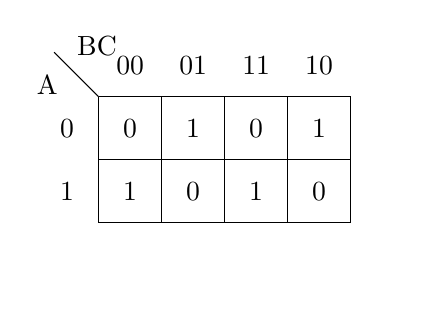
\begin{tikzpicture}[baseline=(current bounding box.north),scale=0.8]
\draw (0,0) grid (4,2);
\draw (0,2) -- node [pos=0.7,above right,anchor=south west] {BC} node [pos=0.7,below left,anchor=north east] {A} ++(135:1);
%
\matrix (mapa) [matrix of nodes,
column sep={0.8cm,between origins},
row sep={0.8cm,between origins},
every node/.style={minimum size=0.3mm},
anchor=4.center,
ampersand replacement=\&] at (0.5,0.5)
{
	\& |(c00)| 00         \& |(c01)| 01         \& |(c11)| 11         \& |(c10)| 10         \& |(cf)| \phantom{00} \\
	|(r00)| 0             \& |(0)|  0 \& |(1)|  1 \& |(3)|  0 \& |(2)|  1 \&                     \\
	|(r01)| 1             \& |(4)|  1 \& |(5)|  0 \& |(7)|  1 \& |(6)|  0 \&                     \\
	|(rf) | \phantom{00}  \&                    \&                    \&                    \&                    \&                     \\
};
%
	\end{tikzpicture}
\\
a)
	$$F = AB'C'+A'B'C+ABC+ABC'$$
	
\begin{figure}[H]
\centering
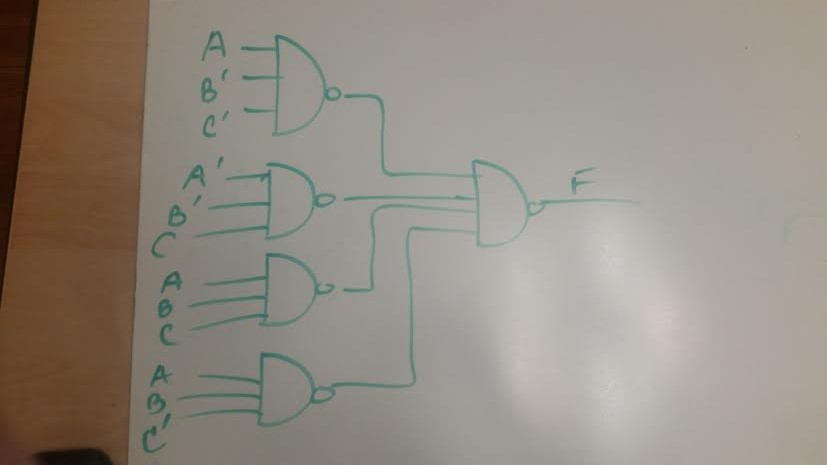
\includegraphics[width=1\linewidth]{nand}
\caption{NAND Gate Implementation}
\label{fig:nand}
\end{figure}
~\\	
b) $$F = (A+B+C)(A+B'+C')(A'+B+C')(A'+B'+C)$$
\begin{figure}[H]
\centering
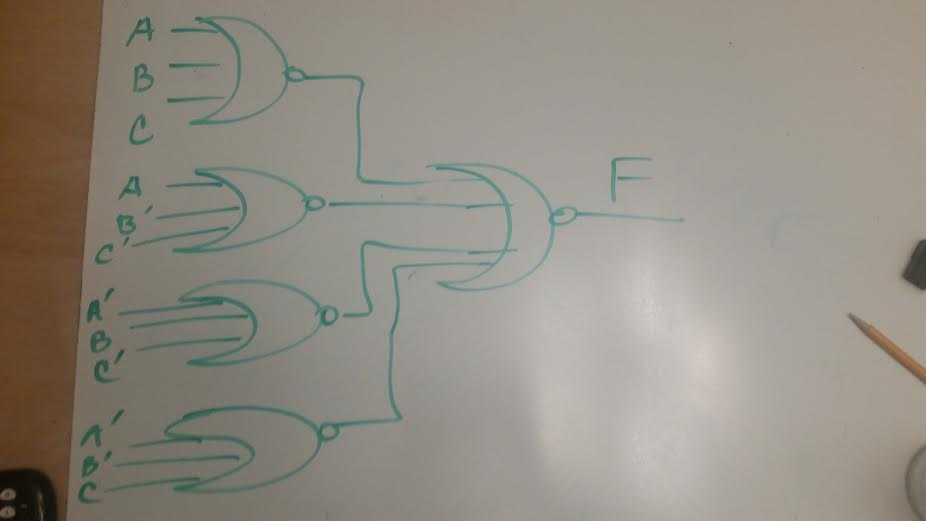
\includegraphics[width=0.9\linewidth]{nor}
\caption{NOR Gate Implementation}
\label{fig:nor}
\end{figure}

\section{CMOS Compound Gate}
a)
\begin{figure}[H]
\centering
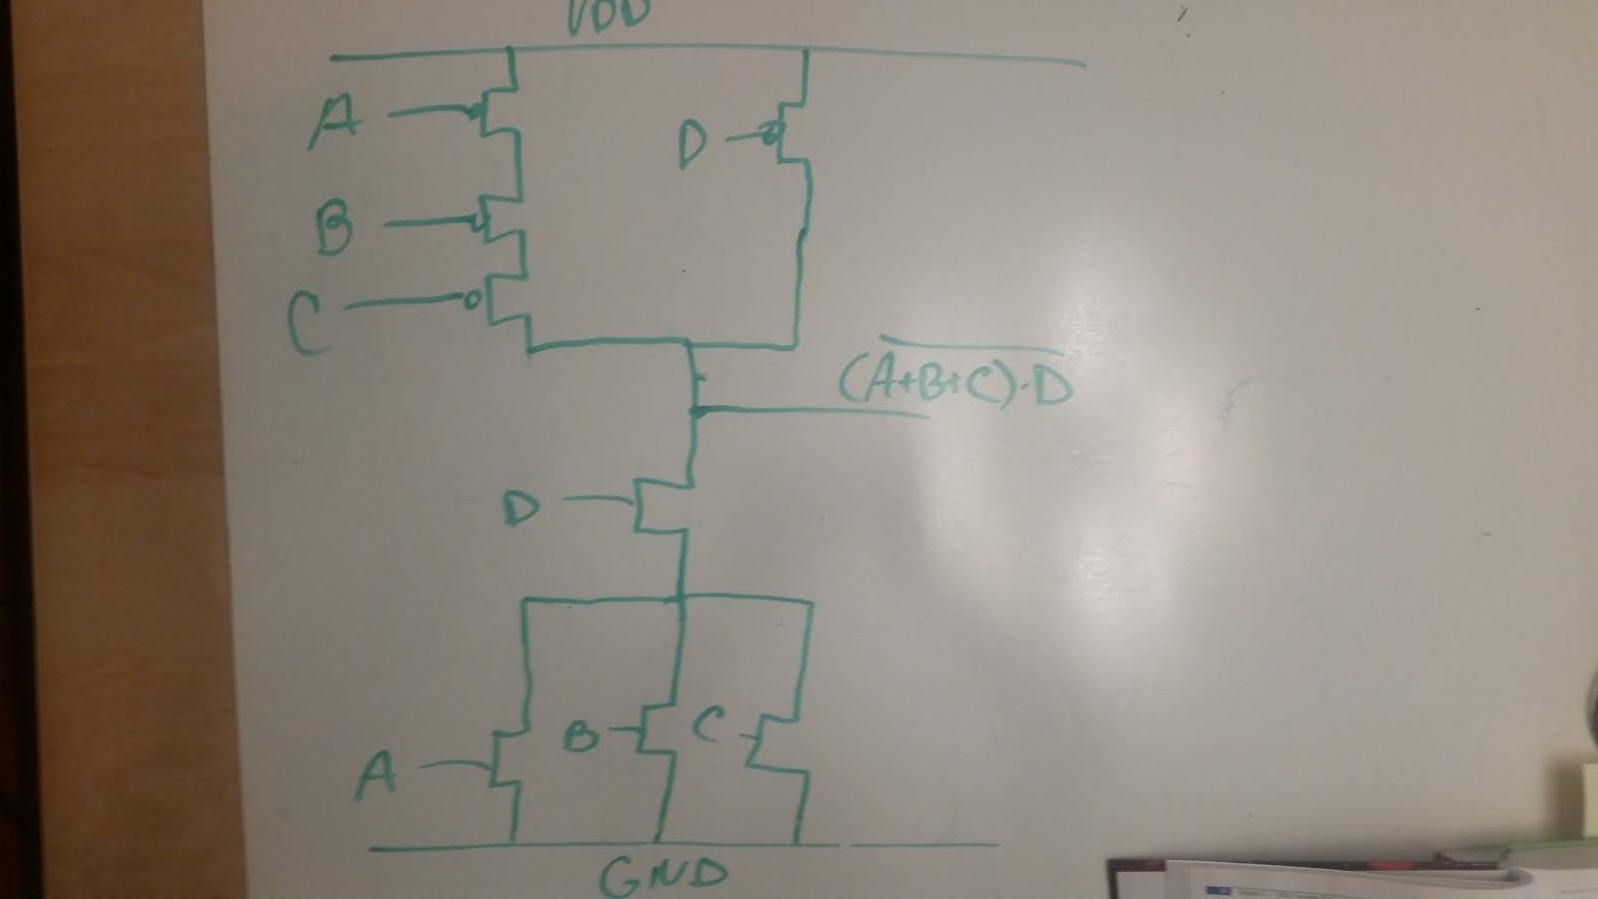
\includegraphics[width=0.9\linewidth]{compound-cmos}
\caption{Transistor-Level Circuit}
\label{fig:compound-cmos}
\end{figure}
~\\
b)
\begin{figure}[H]
\centering
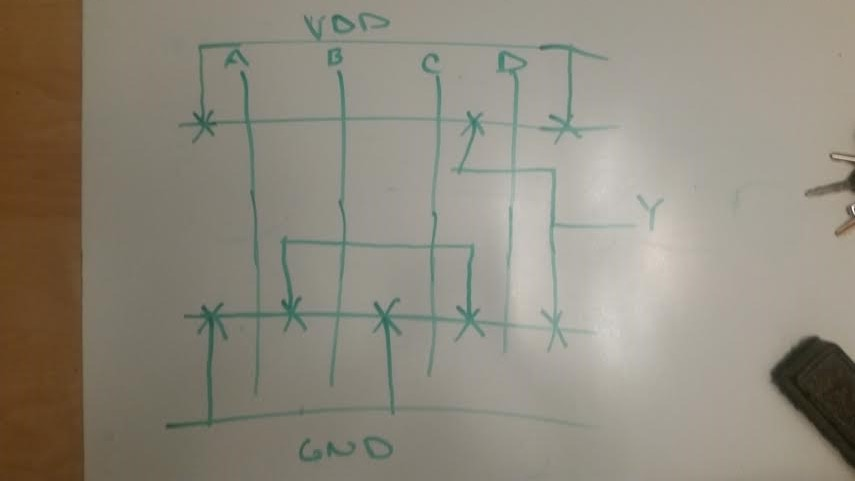
\includegraphics[width=0.9\linewidth]{compound-stick}
\caption{Stick Diagram}
\label{fig:compound-stick}
\end{figure}
~\\
c)\\ 
\indent Height = 6 tracks $\times$ 8$\lambda$ = 48$\lambda$\\
\indent Width = 5 tracks $\times$ 8$\lambda$ = 40$\lambda$

\end{document}
